\documentclass{article}
\usepackage{amssymb}
\usepackage{amsmath}
\usepackage{mathtools}
\usepackage{graphicx} % Required for inserting images
\usepackage{parskip}
\graphicspath{ {./imagens/} }
\usepackage[a4paper, total={7in, 10in}]{geometry}
\usepackage{mathtools} %box inside align
\newcommand\cha{4}
\title{Capítulo \cha\   - Sutton}
\author{Paulo Henrique Albuquerque}
\date{2023-04-25}


\setlength{\parskip}{1ex} % espaçamento vertical entre parágrafos
\setlength{\parindent}{0pt} % recuo horizontal de parágrafos


\begin{document}

\maketitle

\section{Programação Dinâmica}
Algoritmos clássicos de programação dinâmica são de uso limitado pois eles assumem um modelo perfeito, além de terem um grande custo computacional.

Porém, os algoritmos de DP formam uma base essencial para entender outros métodos. Esses outros métodos geralmente tentam replicar os algoritmos de DP com menos computação e sem assumir um modelo ideal. O objetivo primário dos algoritmos de DP é computar funções valor.

\subsection{Avaliação de Política}
Consideramos o problema de calcular $v_{\pi}$ para um política $\pi$ arbitrária. Lembre-se de que,
\[
  v_{\pi}(s)=\sum_{a}^{} \pi(a|s) \sum_{s',r}^{} p(s',r|s,a)[r+\gamma v_{\pi}(s')]
.\] 

A equação acima representa um sistema linear de $|\mathcal{S}|$ equações lineares, que pode ser resolvido atráves de uma computação direta. Para os nossos propósitos, um método interativo é mais adequado. Considere uma sequência de aproximações para a função valor: $v_1,v_2,\ldots$. A primeira aproximação é escolhida de forma arbitrária (exceto para estados terminais, que devem ter valor 0), e cada aproximação sucessiva é obtida usando a equação de Bellman como uma regra de atualização:
\[
  v_{k+1}(s)=\mathbb{E}_{\pi}[R_{t+1}+\gamma v_{k}(S_{t+1})|S_t=s]=\sum_{a}^{} \pi(a|s) \sum_{s',r}^{} p(s',r,|s,a)[r+\gamma v_{k}(s')],
\] 
para todo $s \in \mathcal{S}$. Claramente, $v_{\pi}$ é um ponto fixo para essa regra de atualização, pois a equação de Bellman garante a igualdade nesse caso. De fato, a sequência $\{v_{k}\}$ converge para $v_{\pi}$ a medida que  $k \to \infty$ sob as mesmas condições que garantem a existência de $v_{\pi}$. Esse algorimo é chamado de \textit{avaliação iterativa de política}.

Na implementação do algoritmo podemos utilizar um array e atualizar os valores in place. Pode-se ser, então, que novos valores sejam usados em vez de valores antigos no lado direito da equação da regra de atualização. Essa algoritmo levemente modificado também funciona e, usualmente, converge mais rápido. Geralmente, utilizamos a versão in place quando pensamos em algoritmos de DP.

O algoritmo de avaliação iterativa de política é dado abaixo.

\begin{figure}[htpb]
  \centering
  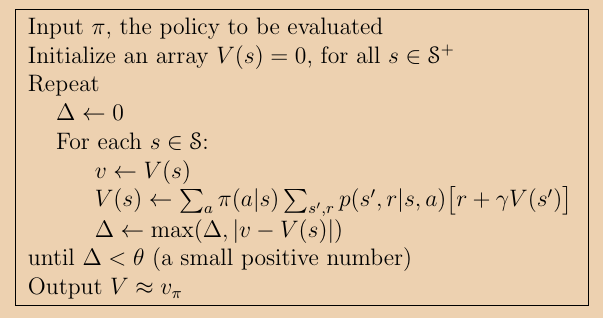
\includegraphics[width=0.4\textwidth]{fig4.1.png}
  \caption{Algoritmo de avaliação iterativa de política}
  \label{fig:}
\end{figure}

\newpage

\subsection{Melhoria de política}  
Para sabermos se uma política pode ser melhorada comparamos o valor de $v_{\pi}(s)$ com $q_{\pi}(s,a)$ para toda ação $a \in \mathcal{A}(s)$. Caso algum $q_{\pi}(s,a)$ seja maior que $v_{\pi}(s)$, a política pode ser melhorada dando preferência à ação $a$ quando o agente está no estado $s$. Anunciamos essa observação através do seguinte teorema.

Melhoria de política: Sejam $\pi$ e $\pi'$ duas políticas determinísticas tais que, para todo $s \in \mathcal{S}$,
\[
  q_{\pi}(s,\pi'(s)) \ge v_{\pi}(s)
.\] 

Então, a política $\pi'$ é tão boa quanto $\pi$, ou até melhor:
\[
  v_{\pi'}(s) \ge v_{\pi}(s)
,\] 
para todo $s \in \mathcal{S}$. Podemos estender essa argumentação para todos os estados. Então, para cada estado, procuramos a ação que maximize o retorno:
\[
  \pi'=\arg \max_{a} q_{\pi}(s,a)=\sum_{s',r}^{} p(s',r|s,a)[r+\gamma v_{\pi}(s')]
.\] 
O processo de construir uma nova política melhorada, ao fazê-la gulosa em relação às funções valor da política original, é chamado de \textit{melhoria de política}.

Suponha que ao construir uma nova política $\pi'$ através da melhoria de política, obtemos uma política não melhor que $\pi$. Ou seja, $v_{\pi'} = v_{\pi}$. Pela equação acima, segue que, para todo $s \in \mathcal{S}$:
\[
  v_{\pi}(s')=\max_{a} \sum_{s',r}^{} p(s',r|s,a)[r+\gamma v_{\pi'}(s')]
.\] 
Mas a equação acima é idêntica à equação de Bellman ótima. Ou seja, $v_{\pi'}=v_{\pi}=v_{\star}$. 

Até agora, consideramos políticas determinísticas. Ao considerarmos políticas estocásticas, basta fazermos a seguinte modificação natural:
\[
  q_{\pi}(s,\pi'(s))=\sum_{a}^{} \pi'(a|s)q_{\pi}(s,a)
.\] 

Além disso, se várias ações são maximizadoras, não precisamos selecionar somente uma ação. Cada ação dessas pode ser dada uma porção da probabilidade de ser selecionada na nova política gulosa. É claro que toda ação sub-maximal deve ter probabilidade zero.

\newpage

\subsection{Iteração de política}
A partir do momento que uma política $\pi$ foi melhorada usando $v_{\pi}$ para obter uma política melhorada $v_{\pi'}$, podemos então computar $v_{\pi'}$ e melhora-lá denovo para obter uma política ainda melhor $\pi''$. Podemos, portanto, obter uma sequência de políticas monotonicamente melhoradas e funções valor:
\[
  \pi_0 \xlongrightarrow[]{\text{E}} v_{\pi_0} \xlongrightarrow[]{\text{I}} \pi_1 \xlongrightarrow[]{\text{E}} v_{\pi_1} \xlongrightarrow[]{\text{I}} \pi_2 \xlongrightarrow[]{\text{E}} \ldots \xlongrightarrow[]{\text{I}} \pi_{\star} \xlongrightarrow[]{\text{E}} v_{\star} 
,\] 
onde $\xlongrightarrow[]{\text{E}}$ denota uma avaliação de política e $\xlongrightarrow[]{\text{I}}$ denota uma melhoria de política. Cada política é, garantidamente, uma melhoria estrita em relação à passada se não for uma política ótima. Para MDPs finitos, o processo converge para uma política ótima em um número finito de passos, visto que o número de políticas é finito. (Porque? Só para políticas determinísticas, não?). Veja o algoritmo abaixo.

\begin{figure}[htpb]
  \centering
  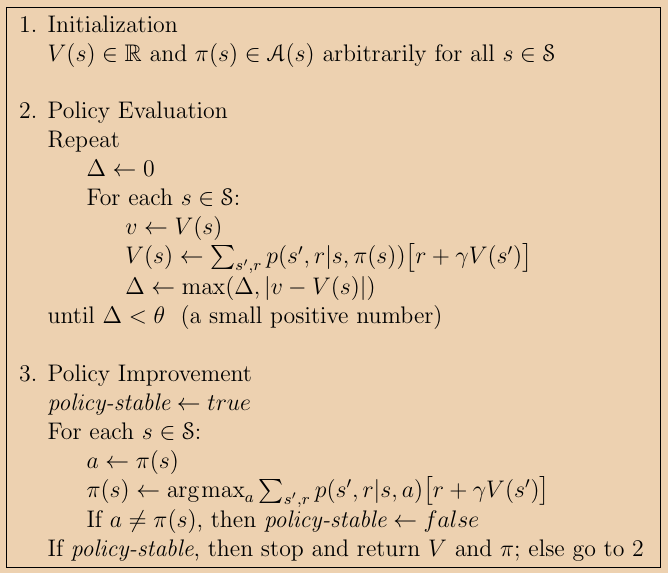
\includegraphics[width=0.4\textwidth]{fig4.3.png}
  \caption{Algoritmo de iteração de políticas}
  \label{fig:fig4-3-png}
\end{figure}


Observe que há um bug. É possível que o algoritmo acima nunca termine, quando o processo fica alterando entre duas políticas igualmente boas (como isso é possível?). Note também que em cada avaliação de política, a função valor é inicializada com o valor da função da política anterior. Isso faz que o processo, em geral, convirga mais rapidamente.

\subsection{Jack's Car Rental}
Nessa seção, fazemos uma apresentação do problema \textit{Jack's Car Rental} junto com sua solução.

O problema consiste 
\end{document}
